\documentclass[12pt,
border=1pt]{standalone}
\usepackage{pgfplots}
\usepackage{amsmath}
\usepackage{amssymb}

\pgfplotsset{compat=newest,
	width=6cm, height=5cm,
	xtick pos=left, ytick pos=left,
	%            scaled x ticks=real:1e-6,
}
% Kernel 2 FP64
\begin{document}
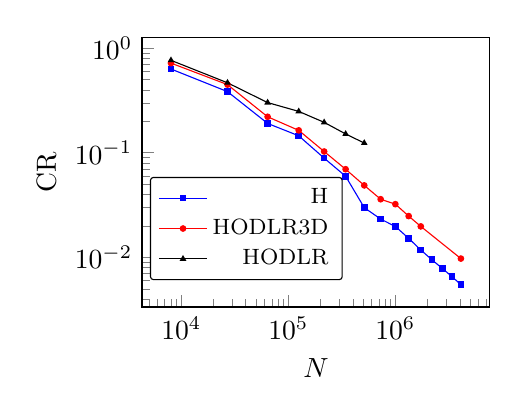
\begin{tikzpicture}[every mark/.append style={mark size=1pt}]
	\begin{axis}[xlabel={$N$},
	ylabel={CR},
%		legend pos=south east,
		legend style={
                at={(0.3,0.1)},
               anchor=south,
               legend columns=1,
               cells={anchor=east},
               font=\footnotesize,
               rounded corners=1pt,
               },
		xmode = log,
	    ymode = log,
	   % xmin = 1e3,
	   % xmax = 1e6,
	   % ymin = 1e-10,
	   % ymax = 1e-0,
	   % xtick={1e-10, 1e-8, 1e-6,  1e-4,  1e-2},
	   % ytick={1e-8, 1e-6,  1e-4,  1e-2, 1e-0}
		]

		%Vaishnavi
		\addplot[
		color=blue,
		mark=square*,
		] coordinates {
(8000,0.632226)
(27000,0.384119)
(64000,0.190866)
(125000,0.145229)
(216000,0.088868)
(343000,0.059626)
(512000,0.029894)
(729000,0.023235)
(1000000,0.019757)
(1331000,0.015216)
(1728000,0.011771)
(2197000,0.009486)
(2744000,0.007843)
(3375000,0.006558)
(4096000,0.005491)
% (4913000,0.004767)
% (5832000,0.004179)
% (6859000,0.003701)
		};
		%Zhao
		\addplot[
		color=red,
		mark=*,
		] coordinates {
(8000,0.719382)
(27000,0.448290)
(64000,0.220833)
(125000,0.163754)
(216000,0.102847)
(343000,0.069620)
(512000,0.048761)
(729000,0.035969)
(1000000,0.032270)
(1331000,0.024819)
(1728000,0.019779)
(4096000,0.009739)
		};
\addplot[
		color=black,
		mark=triangle*,
		] coordinates {
(8000,0.765451)
(27000,0.466623)
(64000,0.301861)
(125000,0.248619)
(216000,0.195355)
(343000,0.151355)
(512000,0.123864)
		};
		\legend{H, HODLR3D, HODLR}	\end{axis}
\end{tikzpicture}
\end{document}